\section{Dataset Riesby}
\subsection{Desenho do Estudo}
\begin{frame}{Dataset Riesby}
    \begin{block}{Sobre o conjunto de dados}
    	\begin{itemize}
    		\justifying
    		\item O dataset Riesby representa um ensaio clínico psiquiátrico longitudinal descrito em Reisby et al. (1977) para tratamento de depressão.
    		\item O estudo focou na relação longitudinal entre os níveis plasmáticos de imipramina (IMI) e desipramina (DMI) e a resposta clínica em 66 pacientes internados com depressão é a mudança nas pontuações de depressão semana a semana.
    		\item Como a imipramina se biotransforma no metabólito ativo desmetilimipramina (ou desipramina), a medição da desipramina também foi feita neste estudo.
    	\end{itemize}
    \end{block}
\end{frame}

\begin{frame}{Desenho do Estudo}
	\begin{block}{Fase Inicial}
		Período de Placebo 
	\end{block}
	\begin{block}{Tratamento}
		Doses de 225mg/dia de imipramina por 4 semanas.
	\end{block}
	\begin{block}{Avaliação}
		Escala de classificação de depressão de Hamilton (Hamilton, 1960).
	\end{block}
	\begin{block}{Medições}
		Nível plasmático de imipramina (IMI) e seu metabólito desipramina (DMI) medidos no final de cada semana de tratamento.
	\end{block}
\end{frame}

\begin{frame}{Desenho do Estudo}
	\begin{block}{Coleta de dados}
		\begin{itemize}
			\item Sexo
			\item Diagnóstico de Depressão: Endógena ou Reativa (Não endógena).
		\end{itemize}
	\end{block}
\end{frame}

\begin{frame}{Desenho do Estudo}
	\begin{block}{Número de Participantes}
		Um total de 66 indivíduos sendo a variação por semana dada por:
		\begin{itemize}
			\item Semana 0: 61 participantes.
			\item Semana 1: 63 participantes.
			\item Semana 2: 65 participantes.
			\item Semana 3: 58 participantes.
		\end{itemize}
	\end{block}
\end{frame}

\begin{frame}{O conjunto de dados}
	\begin{table}[ht]
		\centering
		\caption{Níveis plasmáticos de imipramina (IMI) e desipramina (DMI) e HDRS score em pacientes com depressão durante o tratamento psiquiátrico.}
		\resizebox{\textwidth}{!}{ % 
			\begin{tabular}{crccccc}
				\toprule
				ID & Score (HDRS) & Semana & Sexo & Endógena & IMI(mg/L) & DMI(mg/L) \\
				\midrule
				101 & -8 & 0 & 0 & 0 & 4,043050 & 4,204690 \\
				101 & -19 & 1 & 0 & 0 & 3,931830 & 4,812180 \\
				101 & -22 & 2 & 0 & 0 & 4,330730 & 4,962840 \\
				101 & -23 & 3 & 0 & 0 & 4,369450 & 4,962840 \\
				103 & -18 & 0 & 1 & 0 & 2,772590 & 5,236440 \\
				 $\vdots$ & $\vdots$ & $\vdots$ & $\vdots$ &  $\vdots$ & $\vdots$ & $\vdots$ \\
				360 & 12 & 3 & 0 & 1 & 3,637590 & 4,844190 \\
				361 & -19 & 0 & 1 & 1 & 4,204690 & 3,784190 \\
				361 & -22 & 1 & 1 & 1 & 4,584970 & 4,234110 \\
				361 & -23 & 2 & 1 & 1 & 4,382030 & 4,189650 \\
				361 & -11 & 3 & 1 & 1 & 4,624970 & 4,189650 \\
				\bottomrule
			\end{tabular}
		}
	\end{table}

\end{frame}

\begin{frame}{O conjunto de dados}
	\begin{block}{Questões de Interesse}
		\begin{itemize}
			\item O tratamento obteve resultados satisfatórios?
			\item O tratamento em pacientes endógenos é mais eficaz?
		\end{itemize}
	\end{block}
\end{frame}


\begin{frame}{O conjunto de dados}
	\begin{table}[ht]
		\centering
		\caption{Escore HDRS dos pacientes em cada semana de tratamento.}
		\resizebox{0.5\textwidth}{!}{ % 
			\begin{tabular}{crrrr}
				\toprule
				Semana & 0 & 1 & 2 & 3 \\
				ID &  &  &  &  \\
				\midrule
				101 & -8 & -19 & -22 & -23 \\
				103 & -18 & -9 & -18 & -20 \\
				104 & -11 & -16 & -10 & -29 \\
				105 & -6 & -6 & -9 & -13 \\
				$\vdots$ & $\vdots$ & $\vdots$ & $\vdots$ &$\vdots$ \\
				607 & 0 & -3 & -10 & -26 \\
				608 & -10 & -12 & -21 & -20 \\
				609 & -3 & -11 & -10 & -23 \\
				610 & -1 & -11 & N/A & -23 \\
				\bottomrule
			\end{tabular}
			
		}
	\end{table}
	
\end{frame}


\begin{frame}{Medidas de Resumo}
	\begin{table}[ht]
		\centering
		\caption{Medidas de resumo do Score de Depressão HDRS para cada sexo nas diferentes semanas de tratamento.}
		\resizebox{\textwidth}{!}{ % 
			\begin{tabular}{lccrrrrrrr}
				\toprule
				&  & Quantidade & Média & DP & Min & Q1 & Mediana & Q3 & Max \\
				\hline
				Sexo & Semana &  &  &  &  &  &  &  &  \\
				\midrule
				\multirow[t]{4}{*}{Feminino} & 0 & 19 & -2,79 & 5,24 & -13 & -6,00 & -3,0 & 0,00 & 8 \\
				& 1 & 19 & -6,58 & 8,49 & -24 & -11,00 & -5,0 & -2,00 & 8 \\
				& 2 & 19 & -9,58 & 8,21 & -23 & -15,00 & -9,0 & -4,00 & 7 \\
				& 3 & 18 & -10,67 & 8,98 & -23 & -16,75 & -14,5 & -5,25 & 12 \\
				\cline{1-10}
				\multirow[t]{4}{*}{Masculino} & 0 & 45 & -5,80 & 5,23 & -19 & -10,00 & -4,0 & -2,00 & 6 \\
				& 1 & 46 & -7,00 & 5,60 & -22 & -10,00 & -7,0 & -3,00 & 4 \\
				& 2 & 44 & -9,55 & 7,04 & -23 & -12,00 & -10,0 & -6,50 & 6 \\
				& 3 & 40 & -11,4 & 7,44 & -29 & -15,00 & -11,0 & -6,00 & 7 \\
				\cline{1-10}
				\bottomrule
			\end{tabular}
		}
	\end{table}
	
\end{frame}
% Variancias

\subsection{Análise}

\begin{frame}{Gráfico de trajetórias individuais do Score HDRS para cada sexo.}
		
		\centering
		\resizebox{0.8\textwidth}{!}{ % 
			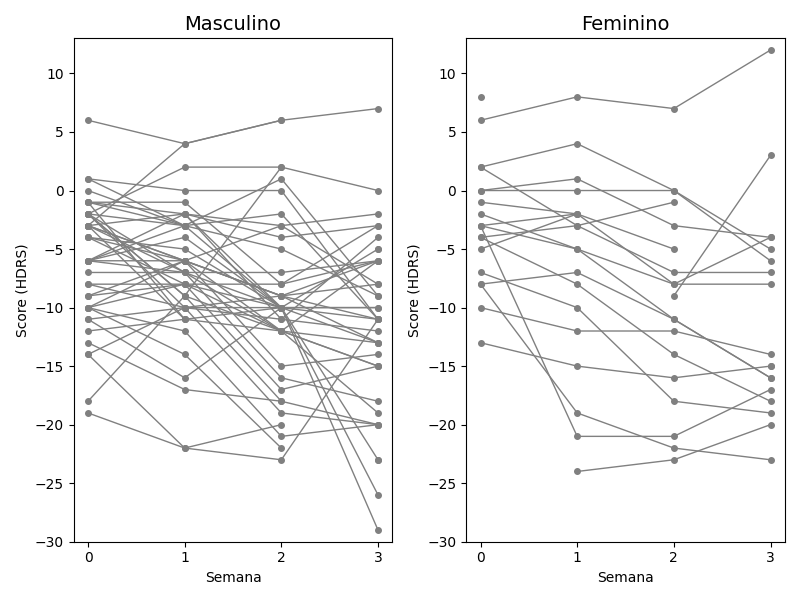
\includegraphics[width=0.7\linewidth]{imagens/secao1/perfis_individuais_por_sexo}
		}

\end{frame}


\begin{frame}{Gráfico de trajetórias individuais do Score HDRS  com perfil médio para cada sexo.}
	
	\centering
	\resizebox{0.8\textwidth}{!}{ % 
		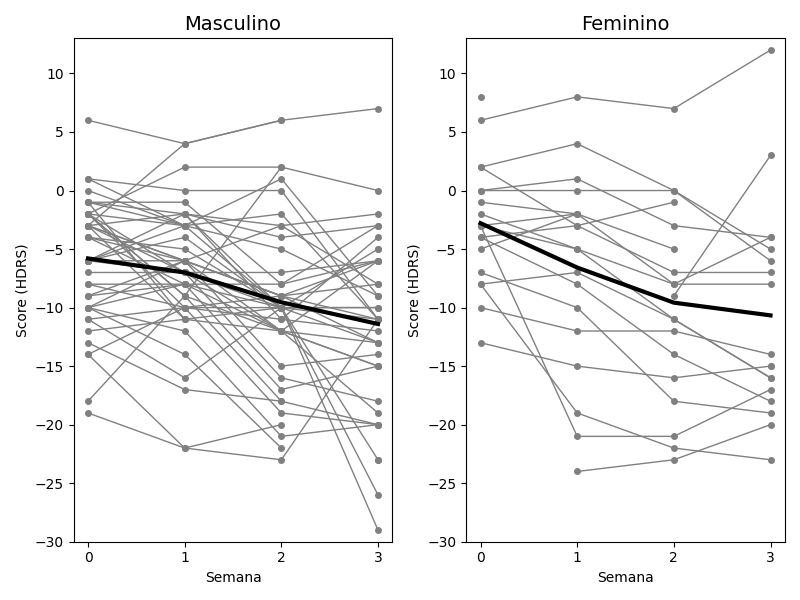
\includegraphics[width=0.7\linewidth]{imagens/secao1/perfis_individuais_por_sexo_com_perfil_medio}
	}
	
\end{frame}

\begin{frame}{Gráfico de trajetórias individuais do Score HDRS  com perfil médio e regressão para cada sexo.}
	
	\centering
	\resizebox{0.8\textwidth}{!}{ % 
		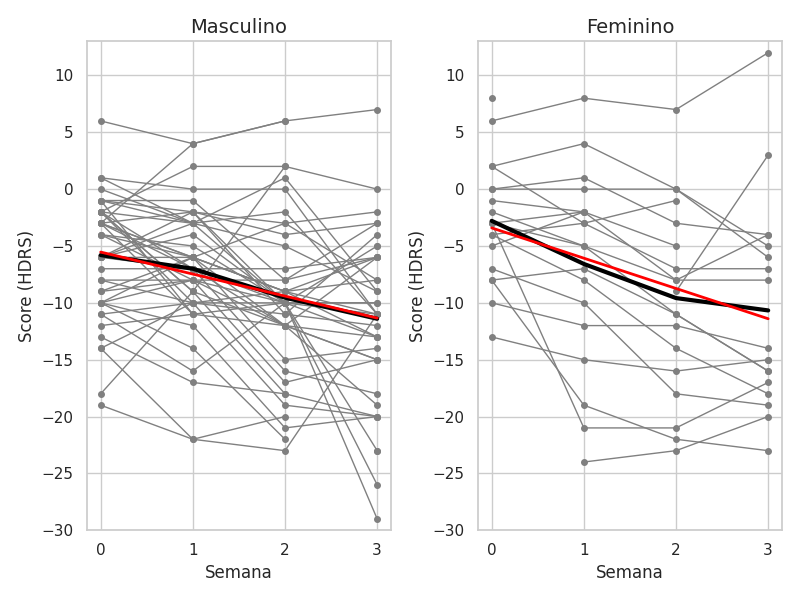
\includegraphics[width=0.7\linewidth]{imagens/secao1/perfis_individuais_por_sexo_com_perfil_medio_e_regressao}
	}
	
\end{frame}

\begin{frame}{Modelos de Regressão simples}
	\begin{block}{Modelo de Regressão para o sexo feminino}
		$$
		y = -3.41 - 2.66x + \varepsilon
		$$
	\end{block}
	\begin{block}{Modelo de Regressão para o sexo masculino}
		$$
		y = -5.53 - 1.93x + \varepsilon
		$$
	\end{block}
\end{frame}

\begin{frame}{}
	Gráfico de trajetórias individuais do Score HDRS para o sexo feminino com perfil médio e regressão simples e regressão polinomial do 2nd grau ajustada.
	\centering
	\resizebox{0.8\textwidth}{!}{ % 
		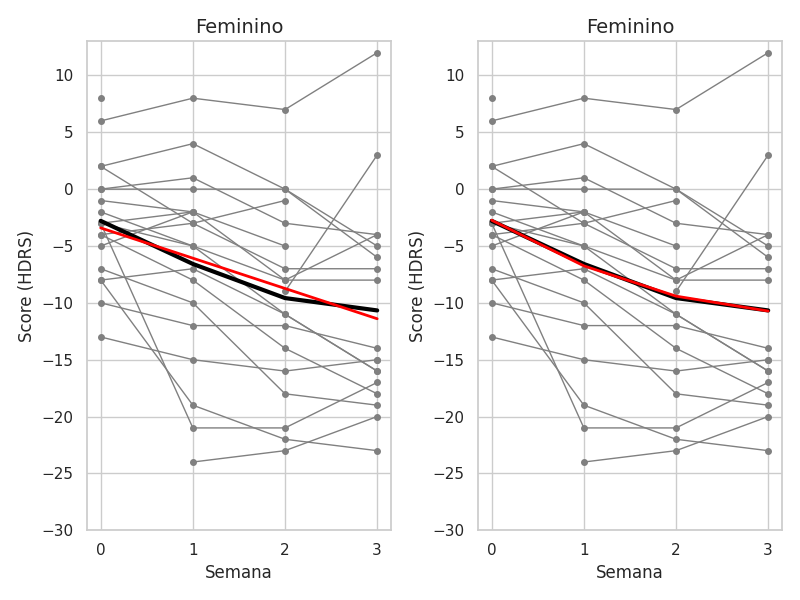
\includegraphics[width=0.7\linewidth]{imagens/secao1/perfis_individuais_por_sexo_com_perfil_medio_e_regressao_ajuste_polinomial}
	}
	
\end{frame}

\begin{frame}{}
	\centering
	\resizebox{\textwidth}{!}{ % 
		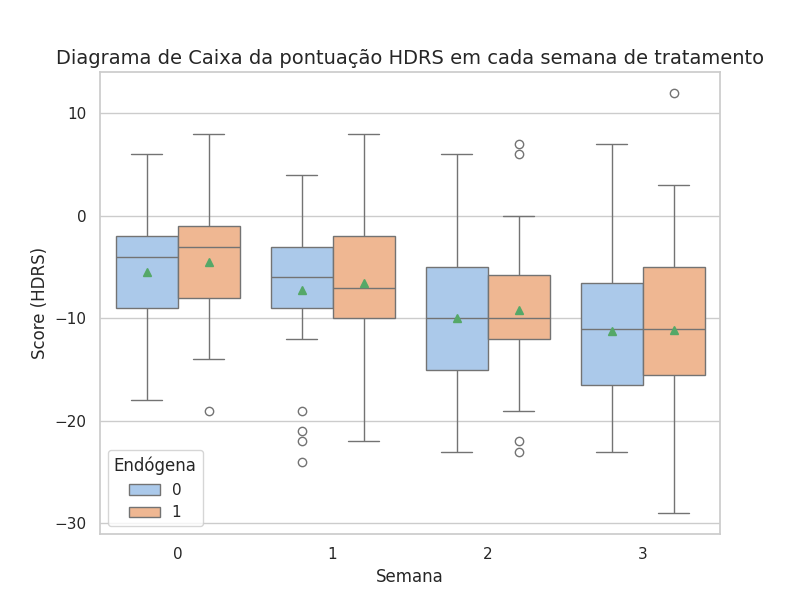
\includegraphics[width=0.7\linewidth]{imagens/secao1/diagrama_de_caixa_pontuacao_HDRS}
	}
	
\end{frame}


\begin{frame}{Regressão via Florestas Aleatórias}
	Para 4 árvores
	\centering
	\resizebox{\textwidth}{!}{ % 
		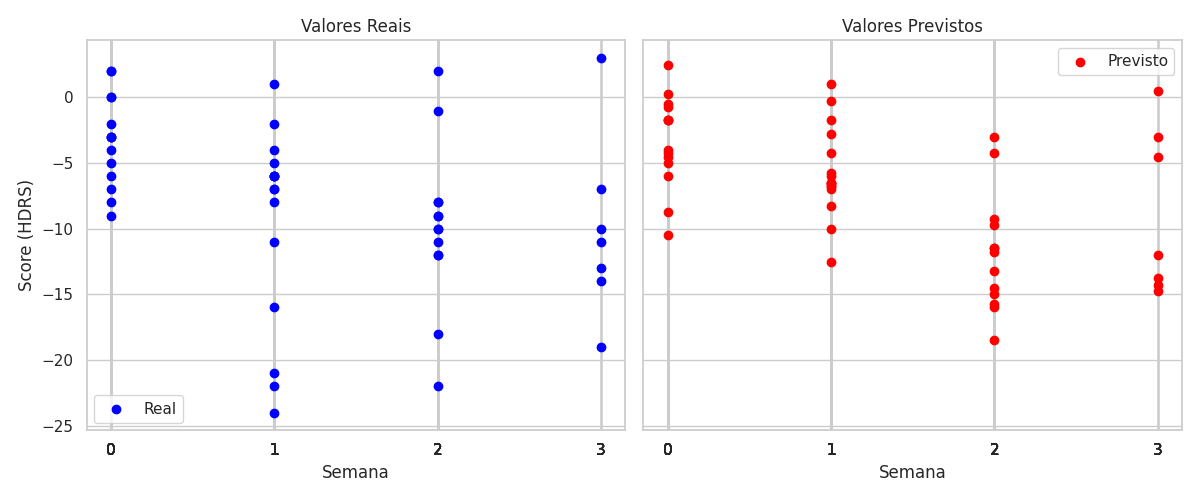
\includegraphics[width=0.8\linewidth]{imagens/secao1/RF_separados_4}
	}
	
\end{frame}

\begin{frame}{Regressão via Florestas Aleatórias}
	Para 10 árvores
	\centering
	\resizebox{\textwidth}{!}{ % 
		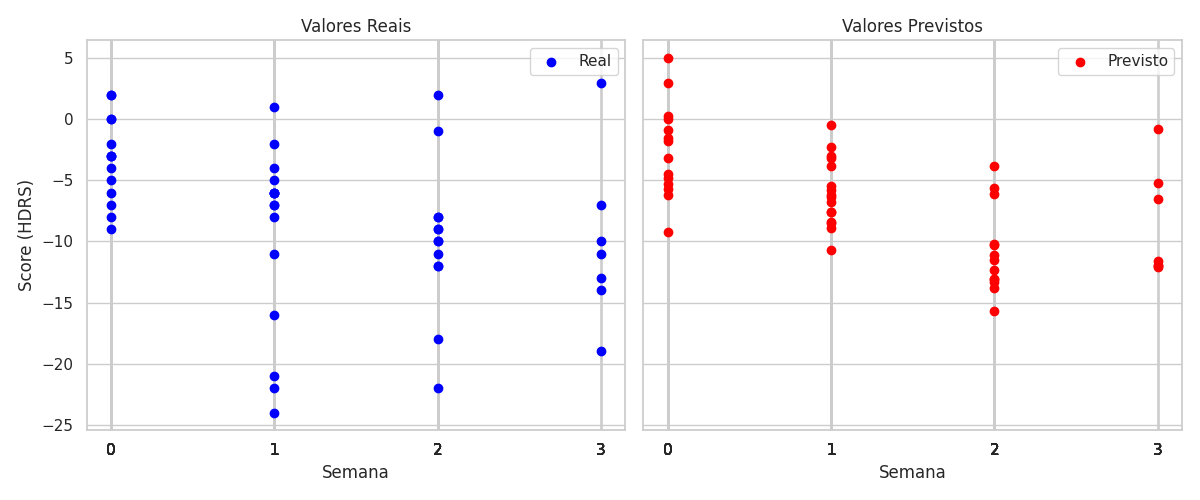
\includegraphics[width=0.8\linewidth]{imagens/secao1/RF_separados_10}
	}
	
\end{frame}

\begin{frame}{Regressão via Florestas Aleatórias}
	Para 50 árvores
	\centering
	\resizebox{\textwidth}{!}{ % 
		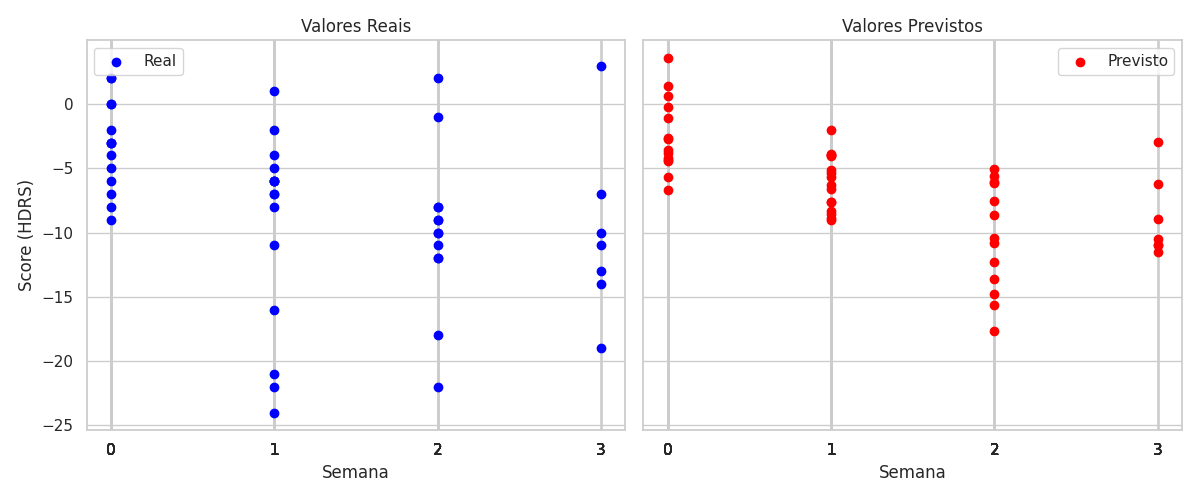
\includegraphics[width=0.8\linewidth]{imagens/secao1/RF_separados_50}
	}
	
\end{frame}

\begin{frame}{Regressão via Florestas Aleatórias}
	Para 100 árvores
	\centering
	\resizebox{\textwidth}{!}{ % 
		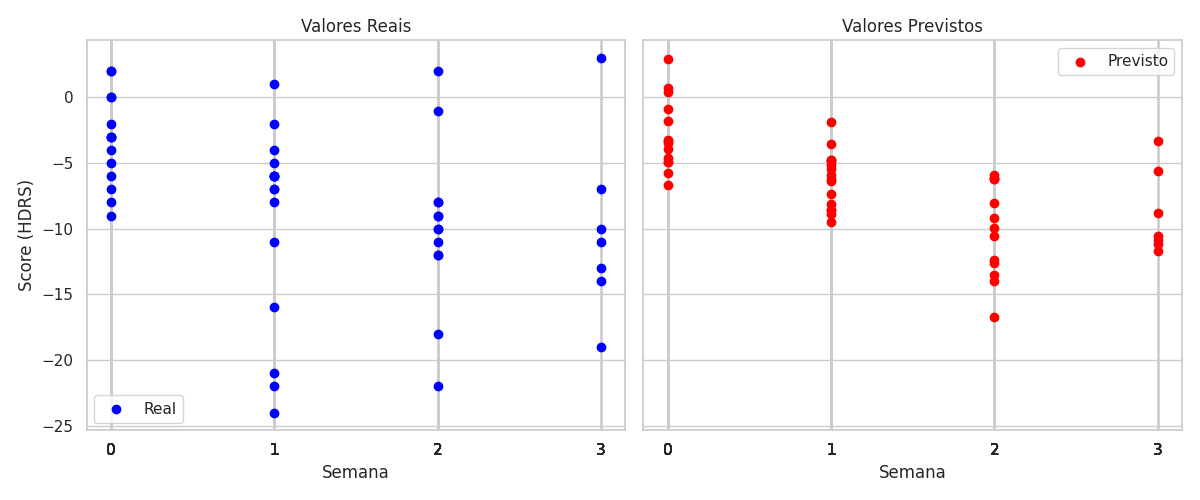
\includegraphics[width=0.8\linewidth]{imagens/secao1/RF_separados_100}
	}
	
\end{frame}

\begin{frame}{Melhor Escolha de Hiperparametro}
\begin{table}[h!]
	\centering
	\caption{Comparação de Hiperparâmetros do Random Forest}
	\begin{tabular}{|c|c|c|c|}
		\hline
		\textbf{Num de Árvores} & \textbf{EQM} & \textbf{$R^2$ Score} & \textbf{EMA} \\
		\hline
		4  & 44.06 & -0.0309 & 5.06 \\
		10 & 31.50 &  0.2630 & 4.33 \\
		50 & 33.30 &  0.2203 & 4.42 \\
		100 & 32.70 &  0.2300 & 4.27 \\
		\hline
	\end{tabular}
\end{table}

\end{frame}



\begin{frame}{Regressão via Florestas Aleatórias}
	\centering
	\resizebox{\linewidth}{!}{ % 
		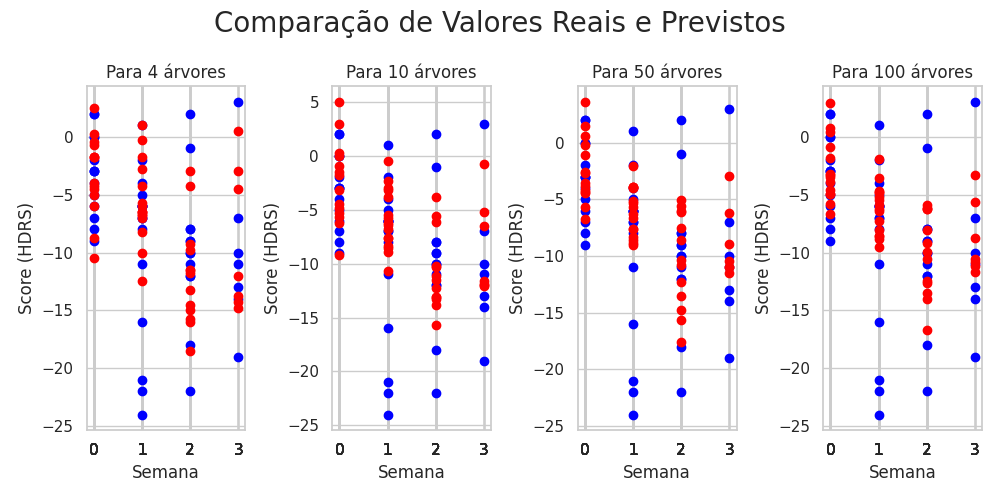
\includegraphics[width=0.6\linewidth]{imagens/secao1/RF_comparação}
	}
	
\end{frame}
